\documentclass{standalone}
\usepackage{tikz}
\usetikzlibrary{positioning}

\tikzset{
	sinesym/.pic = {
	 \draw [domain=0:2, samples=200] plot (\x, {sin(180*\x)/3});}}
\tikzset{
	osc/.pic = {
	 \coordinate (-inleft) at (-0.8,0) ;
	 \coordinate (-inright) at (0.8,0) ;
	 \coordinate (-out) at (0,-1.5) ;
	 \coordinate (-center) at (0,-0.7) ;
	 \coordinate (-right) at (1.3,-.7) ;
	 \coordinate (-left) at (-1.3,-.7) ;
	 \draw (-1.5,0) -- (1.5,0) arc (0:-180:1.5) --cycle;
	 \pic [scale=1/3] at (-.35,-.7) {sinesym};
	 }
	}
\tikzset{
	 play/.pic = {
	 \coordinate (-in) at (0,0.5) ;
	 \coordinate (-out) at (0,-0.5) ;
	 \coordinate (-right) at (1.2,0) ;
	 \coordinate (-left) at (-1.2,0) ;
	 \draw (-1.2,-0.5) rectangle (1.2,0.5) ;
	 \node at (0,0) {Playback} ;
	 }
    }
\tikzset{
	 mic/.pic = {
	 \coordinate (-out) at (0,-0.45) ;
	 \coordinate (-top) at (0,0.15) ;
	 \coordinate (-right) at (0.5,0) ;
	 \coordinate (-left) at (-0.5,0) ;
	 \draw (-0.5,0.15) -- (0.5,0.15) ;
	 \draw (0,-0.15) circle (0.3cm) ;
	 }
    }
	

\begin{document} \sffamily
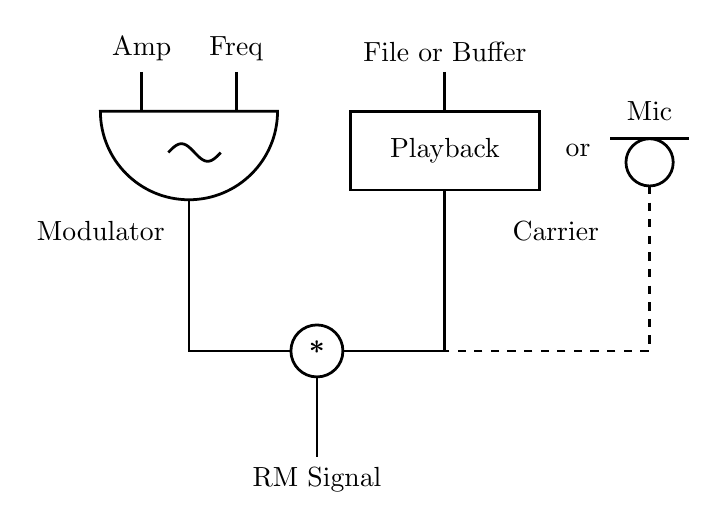
\begin{tikzpicture}[node distance=1, line width=1pt]

% NODES
% carrier
\pic (play) {play};
\node (playin) [above=of play-in, yshift=-0.5cm] {File or Buffer};
\node (or) [right=of play-right, xshift=-0.8cm] {or};
\pic (mic) [right=of play-right, xshift=0.4cm] {mic};
\node [above=of mic-top, yshift=-0.9cm] {Mic};
% modulator
\pic (mod) [scale=3/4, left=of play-in, xshift=-3cm] {osc};
\node (mamp) [above=of mod-inleft, yshift=-0.5cm] {Amp};
\node (mfreq) [above=of mod-inright, yshift=-0.5cm] {Freq};
% mult, output
\path (play-out) -- (mod-out) node (middle) [midway]{};
\node (times) [circle, draw=black, below=of middle, yshift=-.5cm, font=\bfseries] {*};

% label
\node (carlabel) [right=of mod-right, xshift=2cm, yshift=-1cm] {Carrier};
\node (modlabel) [left=of mod-left, xshift=1.8cm, yshift=-1cm] {Modulator};
\node (out) [below=of times] {RM Signal};

%CONNECTIONS
\draw (mamp) -- (mod-inleft);
\draw (mfreq) -- (mod-inright);
\draw (playin) -- (play-in);
\draw (play-out) |- (times);
\draw [dashed] (mic-out) |- (times);
\draw (mod-out) |- (times);
\draw (times) -- (out);

\end{tikzpicture}
\end{document}